\section{Task Definition}

For this bachelor thesis methods for cutting a parachute line shall be investigated. A dedicated device has to be developed and manufactured to separate the parachute lines. The line cutter needs to be light and small enough to be placed inside the parachute as shown in Figure \ref{fig:cutter-placement}. Additionally the device needs to be durable to withstand forces acted on it during the deployment of the parachute.  

The line cutter interfaces through a wireless link, from the body of the rocket, with the main recovery computer. The computer can then initiate the separation of the reefing line. As a backup method, independent operation should also be supported. In that case, air pressure data shall be used to deploy the reefing line at a set altitude.

\begin{figure}[h!]
	\centering
	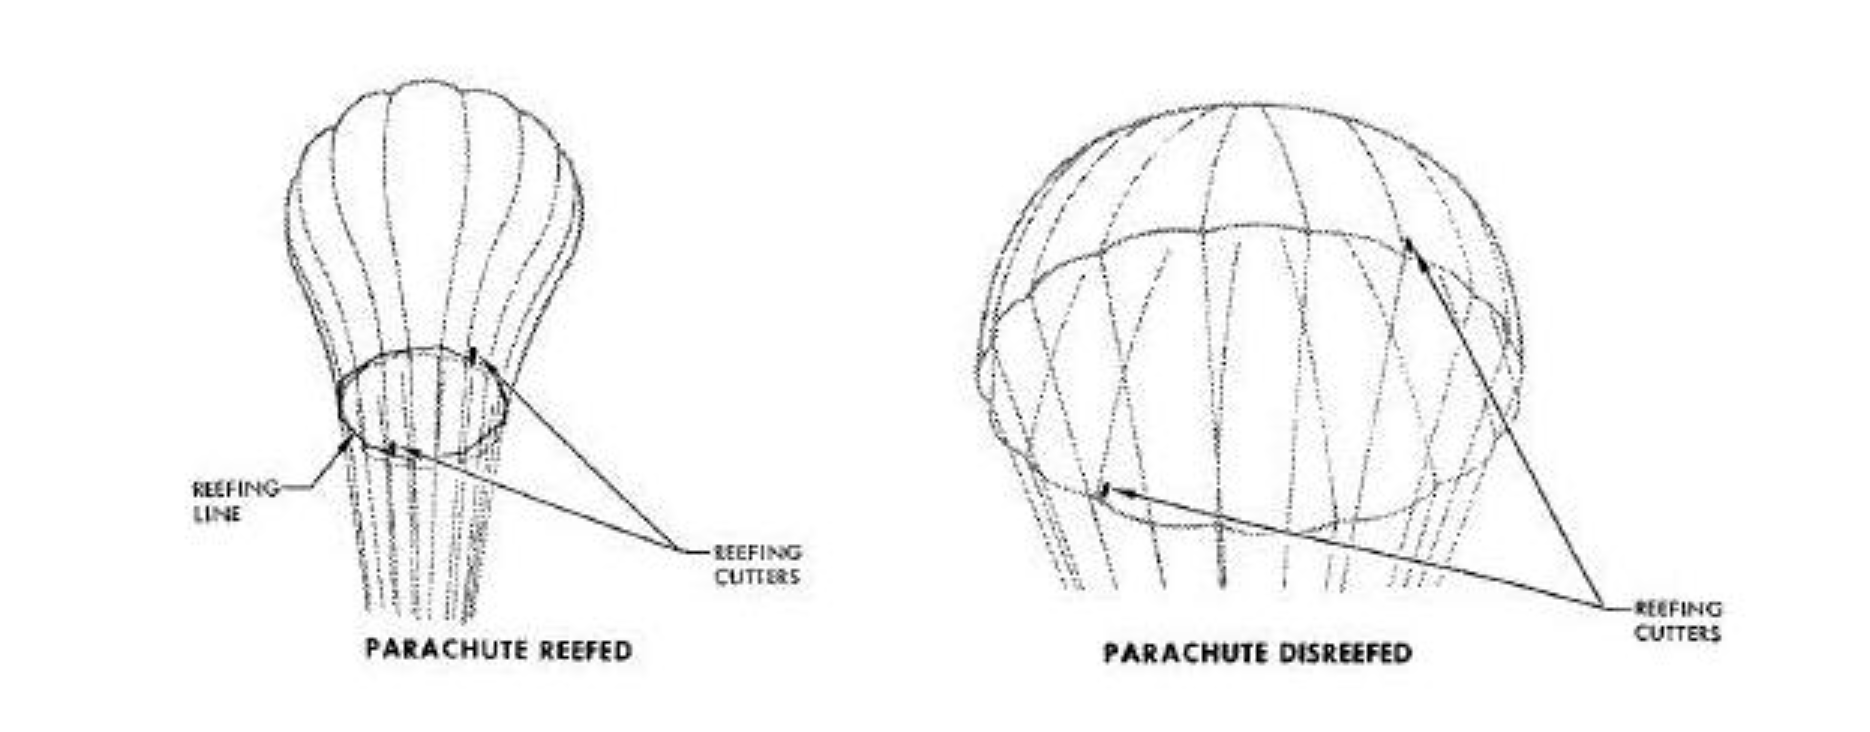
\includegraphics[height=7.3cm]{images/parachute_placement.png}
	\caption{Illustration of line cutter placement from NASA Gemini missions in 1963}
	%\vspace{-2ex}
	\label{fig:cutter-placement}
\end{figure}